%\chapter{det-comp}


%%%%%%%%%%%%%%%%%%%%%%%%%%%%%%%%%%%%%%%%%%%%%%
%\section{Anode Plane Assemblies}

%%%%%%%%%%%%%%%%%%%%%%%%%%%%%%%%%%%%%%%%%%%%%%
\section{Cathode Plane Assemblies}


\subsection{Scope, Requirements and Design Parameters}

The cathode plane is constructed from 6$\times$3 cathode plane assemblies (CPAs) to form the 16m $\times$ 6m area.  It has a HV cup at the beam downstream side to interface with the HV feedthrough. The top and bottom field cage modules are mechanically and electrically connected to the top and bottom edges of the cathode plane.  The cathode plane is suspended through insulating bars to the CPA installation rail.

\subsubsection{Requirements}

\begin{itemize}
\item Provide equipotential surfaces at -180kV nominal bias voltage
\item Maintain a flatness better than 1cm
\item Use materials with comparable CTEs to that of stainless steel 
\item Limit the electric field exposed to LAr to under 30kV/cm
\item Prevent damage to the TPC including its readout electronics In case of a HV discharge anywhere on the cathode
\item Provide constant bias voltage and current to all attached field cage resistor divider chains
\item Support the full weight of the 4 connected top/bottom field cage modules and a person on the bottom CPA at installation
\item Constructed in modular form that can be easily installed in the cryostat
\item Accommodate PD calibration features

\end{itemize}

\subsubsection{Design Parameters}

Width, height, sheet thickness, frame thickness, module width...


\subsection{The need for highly resistive cathode planes}
Stored energy, charge injection to FEE, dominant ionization current density

Summarize key points in DUNE docdb 1320.

\subsection{The design of the CPA modules}

\subsection{Overview}

Introduce the design concept: strong frame with thin resistive cathode surface; field shaping strips cover the frame; HV bus hidden behind the field shaping strips; outer edges of the CPA frame surrounded by the metal profiles used by the field cage.

\begin{cdrfigure}[CPA Concept]{cpa-concept}{The resistive CPA concept. 
 {\bf Left:} A 3d model of a corner of the cathode showing major components {\bf Right:} E field simulation of a portion of the cathode.} 
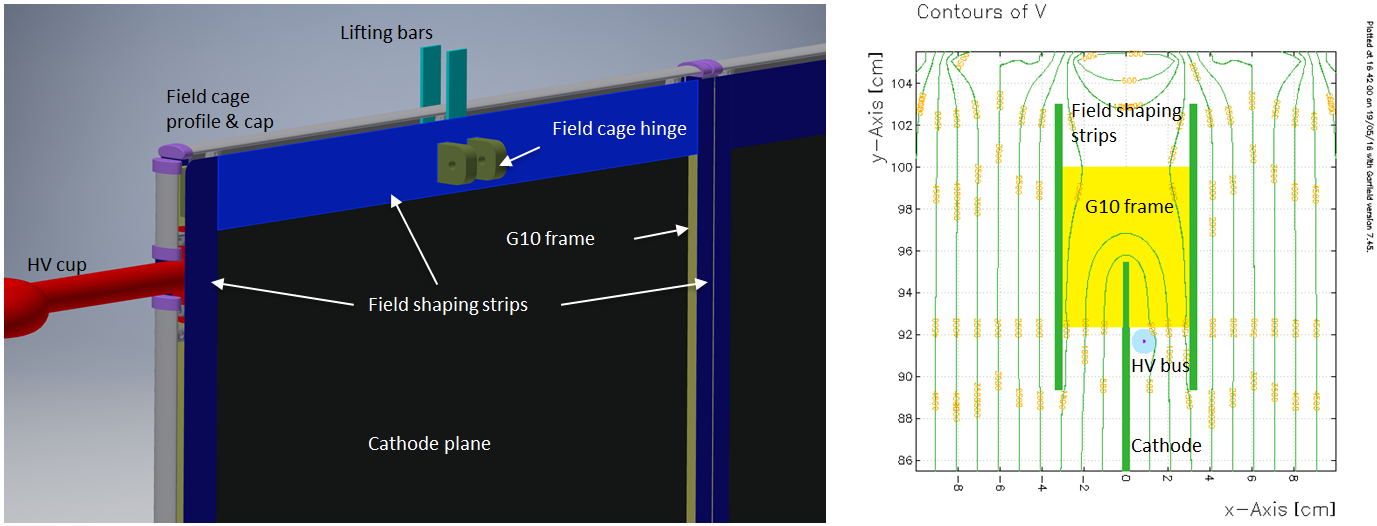
\includegraphics[width=\linewidth]{tpc_cpa_concept.png}
\end{cdrfigure}


\subsubsection{Resistive material}
%% from F. Pietropaolo

The main criteria for the selection of the resistive material to be used for the CPA panels include: 
\begin{itemize}	
\item Surface resistivity range.
\item Compatibility with cryogenic temperatures
\item Robustness to HV discharges, material ageing.
\item Radio-purity.
\item Availability on large area; achievable planarity 
\end{itemize}

Several options have been evaluated.
\begin{itemize}	
\item NORPLEX, Micarta, NP 315, phenolic laminate loaded with graphite: Intrinsic bulk resistivity in the required range (few M$\Omega$/cm). Density comparable to LAr.
\item Screen printed resistive ink on G10/FR4 substrate (~100 k$\Omega$/square) printed with specific patterns to obtain required average surface resistivity
\item DuPont resistive Kapton film  (25 $\mu$m thickness, graphite loaded, available with resistivity in the 0.5 to 50 M$\Omega$/square range) laminated on G10/FR4 substrate.
\end{itemize}
Also considered at earlier stage:
\begin{itemize}	
\item Zelec ESD powder mixed with polyurethane binder.
\item ESD surface conducting G10 from Current Composite.
\end{itemize}

Radiological tests performed at the LNGS low counting rate facility that G10/FR4 are preferable since MiCarta is more active by orders of magnitude for most relevant radioactive chains.
 
Screen printed ink and Kapton lamination on G10/FR4 are well established fabrication techniques available on panels as large as to 2.1x 1.2 m$^2$ (well matching the CPA panel required size). The screen print technique allows to choose precisely the average surface resistivity value, while Kapton exhibits a more uniform surface and resistivity. 

Tests on large size panels have demonstrated that both options survive without deformation or delamination to repeated immersions in LAr. The resistivity increase at LAr temperature is bounded to less than a factor two for both cases. Electrical contacts are performed with  specific  silver paint paste  highly stable at LAr temperature and resistant to mechanical scratches.

Tests on surface ageing when exposed to HV sparks indicate that Kapton is the preferred solution because:
\begin{itemize}	
\item in the resistive ink case, sparks tend to develop along direction of less resistivity, perpendicular to strip direction inducing a visible degradation of the material surface with some consistent ink evaporation and local measurable change in resistivity (Figure~\ref{fig:cpa-resink}).
\item in the Kapton case instead, sparks are point-like inducing tiny localized carbonization on material surface, at the spark position, but no change in average resistivity is recorded (Figure~\ref{fig:cpa-kapton}). 
\end{itemize}

\begin{cdrfigure}[Resistive ink ageing from sparks]{cpa-resink}{Resistive ink ageing from sparks. 
 {\bf Left:} spark propagation along preferred directions (lower resistivity), {\bf Right:} Status after test: degradation with some material evaporation.} 
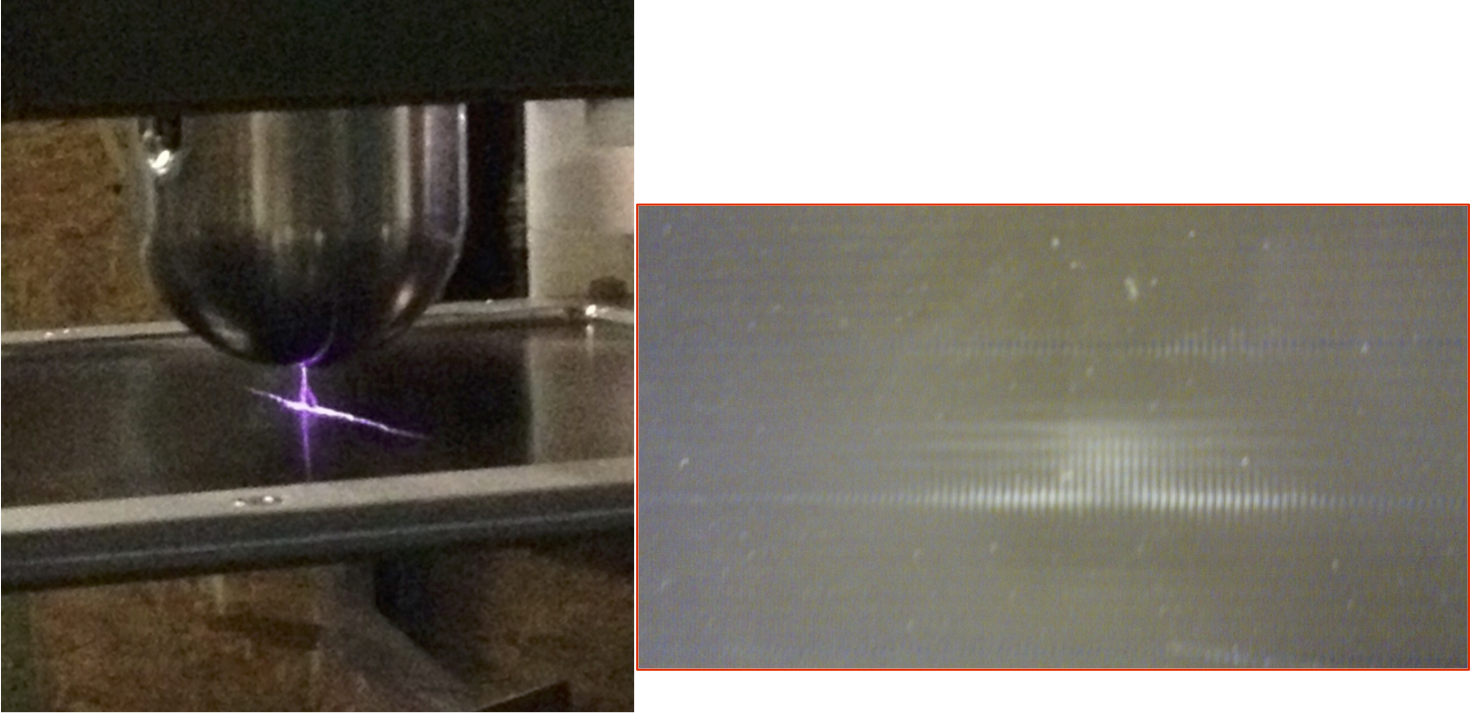
\includegraphics[width=\linewidth]{tpc_cpa-resink.png}
\end{cdrfigure}

\begin{cdrfigure}[The field cage test setup]{cpa-kapton}{Resistive kapton ageing from sparks. 
 {\bf Left:} point-like sparks. {\bf Right:} Localized carbonization on material surface, at the spark position.}
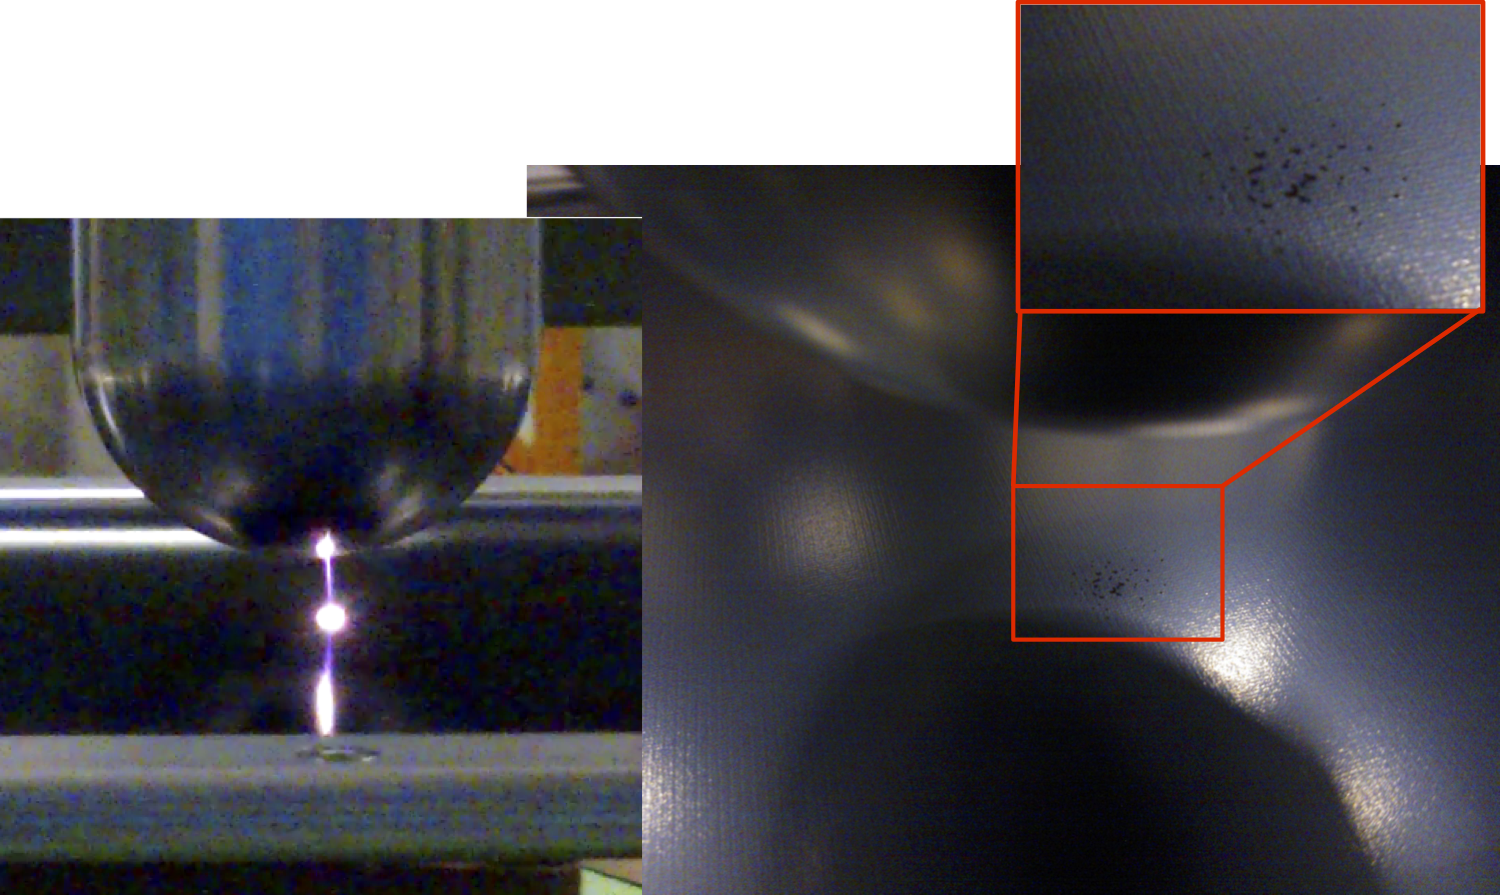
\includegraphics[width=\linewidth]{tpc_cpa-kapton.png}
\end{cdrfigure}

\subsubsection{Support frame structure}

This section will come from Vic's write up.  It includes all the structural analysis due to FD convection flow, FC weight, unbalanced load during FC installation, and personnel load on FC.

\subsubsection{The HV distribution bus and HV feedthrough receptacle }

Should this be moved to the HV section?

\subsubsection{The mechanical and electrical interconnect features between modules}

There are a stack of 3 modules interconnected vertically to form the 6m height of the SP ProtoDUNE cathode.  The frames of these modules are bolted together using tongue and groove connections at the ends, and the resistive cathode sheets, and the field shaping strips are connected  using a few metallic buttons to ensure redundant electrical contact between vertical modules.

There are 6 columns of the 6m tall CPA modules in SP ProtoDUNE.  Each column is suspended to the CPA rail using a central lifting bar.  Due to the  roof movement between the warm and cold phases of the cryostat, each column is expected to move ~ 2mm relative to its neighbors.  Several pin and slot connections are implemented at the long edges of the CPA columns to ensure the co-planarity of the modules and yet allow small vertical displacement.  The HV bus interconnect the resistive cathode surfaces across the columns to maintain a uniform voltage across the cathode surface.


\subsection{Assembly sequence and QC procedures}

\subsection{Installation sequence}




